\documentclass{report}
\usepackage{a4wide}
\usepackage{bm}
\usepackage{amsfonts}
\usepackage{graphicx}
\usepackage{amsmath}

\title{Unsupervised learning for local structure detection in colloidal systems}
\author{Georgios Smyridis, Rimo Sarkar}
\date{}
\begin{document}
\maketitle


\chapter{Introduction}

\section{What are Colloidal Systems?}

\textbf{Colloidal systems}, also known as colloidal suspensions or colloids, are a type of mixture composed of two or more substances. They consist of \textbf{dispersed particles}, typically ranging in size from 1 nanometer to 1 micrometer, suspended in a medium such as a liquid, gas, or solid.

In a colloidal system, the dispersed phase consists of \textbf{colloidal particles}, which can be solid, liquid, or gas-like in nature. These particles are larger than individual molecules but smaller than macroscopic particles. The medium in which the particles are dispersed is called the continuous phase or \textbf{dispersing medium}.

The behavior and properties of colloidal systems are influenced by various factors, including the nature of the particles and the dispersing medium, as well as the interactions between the particles.

Common examples of colloidal systems include milk, paints, ink, fog, aerosols, and gels. In these systems, the colloidal particles are dispersed in a liquid medium. However, colloidal systems can also exist in gas or solid media. For instance, smoke and atmospheric haze are examples of colloidal systems where solid particles are dispersed in a gas medium.

Colloidal systems have diverse applications in various fields. They are utilized in industries such as pharmaceuticals, food and beverage, cosmetics, materials science, and environmental engineering. Colloidal systems play a crucial role in the development of functional materials, drug delivery systems, catalysis, and the stabilization of emulsions and suspensions.

\section{What is local structure in colloidal systems?}

In colloidal systems, \textbf{local structure refers to the arrangement or organization of colloidal particles in the immediate vicinity of an individual particle}.

For example, in a colloidal suspension, the particles can exhibit different types of local structures depending on the balance of attractive and repulsive forces between particles. When the repulsive forces dominate, the particles tend to stay dispersed and form a stable structure called a colloidal fluid or sol. In contrast, when attractive forces become significant, particles can aggregate or cluster together, forming a variety of local structures such as clusters, chains, or even crystalline arrangements.

\section{What is colloidal self-assembly?}

\textbf{Colloidal self-assembly refers to the spontaneous organization of colloidal particles into ordered structures due to their interactions and without external intervention.}

Colloidal self-assembly can lead to the formation of a wide range of structures, including clusters, chains, networks, layers, and even crystalline arrangements. The specific structure that emerges is determined by factors such as particle size, shape, surface properties, and the balance between attractive and repulsive forces.

The self-assembly process can be influenced by external factors such as temperature, concentration, pH, and the presence of additives or solvents. By manipulating these parameters, researchers can set the environment so that the self-assembly process will result to desired structures with specific properties.

\section{Detection of self-assembled products (known phases)}



When the phases/products that the system forms are well-characterised, one can design order parameters that detect, on a single particle level, which of the expected phases the particle is in. This method has been extensively used in the study of crystal nucleation and growth, crystal melting and even grain boundary dynamics. a number of different routes have been taken to characterise such local order, including e.g. order parameters based on bond-orientational order, common neighbor analysis (CNA), and templating.

\subsection{What is crystal nucleation and growth?}


Crystal nucleation and growth are fundamental processes involved in the formation and development of crystalline materials. Crystallization refers to the transformation of a disordered or amorphous material into a highly ordered structure with a well-defined arrangement of atoms or molecules.

\subsubsection{Crystal nucleation}

Crystal nucleation is the initial step in the formation of crystals. It involves the formation of tiny crystal nuclei, which are clusters of atoms or molecules that possess the ordered arrangement characteristic of the crystal lattice. Nucleation can occur spontaneously or be induced by external factors such as temperature, pressure, or the presence of nucleating agents.

During nucleation, the atoms or molecules in the material come together in a favorable arrangement that minimizes the system's free energy. This typically involves the formation of critical clusters, which are small, stable nuclei that can grow into larger crystals. However, the formation of these critical clusters requires overcoming an energy barrier known as the nucleation barrier.


\subsubsection{Crystal growth}

Once the crystal nuclei are formed, they can grow by the addition of atoms or molecules to their surfaces. During crystal growth, atoms or molecules from the surrounding medium attach themselves to the crystal lattice in a specific orientation, resulting in the expansion of the crystal structure.

\subsection{What is grain boundary dynamics}

\subsubsection{Grain boundaries}

Grain boundaries are interfaces or boundaries that separate adjacent crystalline regions, known as grains, in polycrystalline materials. In polycrystalline materials, the grains are individual crystalline structures with different crystallographic orientations.

\subsection{What is bond-orientation order parameter?}
\subsection{What is common neighbour analysis (CNA)?}
\subsection{What is templating?}

\section{Detection of self-assembled products (unknown phases)}

In many cases, when exploring the self-assembly of new systems, the exact final structure and its characteristics are unknown, complicating the selection of an ideal order parameter. In this context, unsupervised machine learning techniques, which excel in autonomously finding patterns in large data sets, offer a promising route for detecting self-assembled structures.

\subsection{Previous works}

There have been a number of methods to detect unknown self-assembled products, recently [Add References].


\chapter{Environment Description}

In this chapter, we describe in detail the algorithm we use to classify local environments. The overall process consists of three steps:
\begin{enumerate}
	\item First, we require a method to capture the local environment of each particle in a set of local order parameters. For this, we make use of bond orientational order parameters. This set of order parameters is in general high-dimensional, and may contain significant amounts of redundant and irrelevant information. In order to extract the most relevant information,
	\item makes use of a dimensionality reduction technique, namely a neural-network-based autoencoder. Once trained, the autoencoder projects the original (high-dimensional) input vectors onto a lower-dimensional subspace encoding the features with the largest variations in the input data. Ideally, in this subspace, particles with similar local environments are grouped together.
	\item Finally, we apply a clustering algorithm (Gaussian mixture models) in order to identify the distinct clusters of local environments in this lower-dimensional subspace.
\end{enumerate}

\section{Bond Order Parameters}

	To characterise the local environment of each particle, we use the averaged bond order parameters (BOPs). For any given particle $i$ we define the complex quantities
	\begin{align}
		q_{lm}(i)=\frac1{N_b(i)}\sum_{j\in\mathcal{N}_b(i)}Y_l^m(\bm{r}_{ij})
	\end{align}
	where $Y_l^m(\bm{r}_{ij})$ are the spherical harmonics of order $l$, with $m$ an integer that runs from $m=-l$ to $m=l$. Additionally, $\bm{r}_{ij}$ is the vector from particle $i$ to particle $j$, and $\mathcal{N}_b(i)$ is the set of nearest neighbours of particle $i$, which we define later. Note that $|\mathcal{N}_b(i)|=N_b(i)$. Then, we define the average $\bar q_{lm}(i)$ as
	\begin{align}
		\bar q_{lm}(i)=\frac1{N_b(i)+1}\sum_{k\in\{i\}\cup\mathcal{N}_b(i)}q_{lm}(k)
	\end{align}
	where the sum runs over all nearest neighbours of particle $i$ as well as particle $i$ itself. Averaging over the nearest neighbour values of $q_{lm}$ results in effectively in also taking next-nearest neighbours into account. Finally, we define rotationally invariant BOPs as
	\begin{align}
		\bar q_l(i)=\sqrt{
		\frac{4\pi}{2l+1}
		\sum_{m=-l}^l|\bar q_{lm}(i)|^2
		}
	\end{align}
	which, depending on the choice of $l$, are sensitive to different crystal symmetries.
	
	The optimal set of BOPs to be considered strongly depends on the structures one wishes to distinguish. Since our method is meant to be applied to systems for which such prior knowledge is missing, in order to describe the local environment of one particle, we evaluate several $\bar q_l$ with $l$ ranging from 1 to 8.
	
	Therefore, when considering one component systems, our description of the local environment of particle $i$ is encoded into an $8$-dimensional vector
	\begin{align}
		\bm{Q}(i)=(\{\bar{q}_l\}),
	\end{align}
	with $l$ integer from 1 to 8.
	
\section{Nearest Neighbours}

When calculating the BOPs, one is confronted with the task of determining the nearest neighbours of a particle. Although performing such task is integral component of various analyses in many particles systems, there is no unique definition of nearest neighbours. One of the most common algorithms for the job is a fixed-distance cutoff algorithm. A fixed-distance cutoff is an obvious choice, and relatively computationally inexpensive. In this algorithm, nearest neighbours of a particle $i$ are the particles that have distance smaller or equal than a threshold. However, the "fixed-distance" is not well-defined. A reasonable choice for a cutoff would arguably be the first minimum of the pair correlation function $g(r)$. However, the precise location of the minimum depends on both the system's details and thermodynamics conditions and therefore must be determined every time either one is changed. Additionally, the cutoff is defined for the entire system and, as such, is not appropriate for systems with large density gradients, i.e. inhomogeneous systems. 

Instead, we have opted to make use of a recently introduced parameter-free nearest-neighbour criterion, called SANN (solid angle nearest neighbour). 




In this approach, an effective individual cutoff is found for every particle in the system based on its local environment. This method is not inherently symmetric, i.e. $j$ might be a neighbour of $i$ while $i$ is not a neighbour of $j$. However, symmetry can be enforced by removing $i$ from the neighbours of $j$. The computational cost of SANN only slightly exceeds that of a cutoff distance, and since it is a parameter-free method, it is suitable for systems with inhomogeneous densities.


\section{}

Consider a system where with have a particle $i$ located at position $\bm{r}_i$ surrounded by particles $\{j\}$. The fixed-distance cutoff defines the nearest neighbours of particle $i$ to be all the particles $\{j\}$ with distance to $i$ smaller than some threshold $R$. i.e.
\begin{align}
	\mathcal{N}_b(i)=\{n:n\in \{j\}\wedge r_{in}\leq R\}
\end{align}
As mentioned above, the problem is choosing the threshold distance $R$. The SANN algorithm provides a solution to this problem by determining an \textit{individual} cutoff distance $R_i^{(m)}$ for each particle $i$, which we call the \textit{shell radius}. This radius depends solely on the local environment of each particle $i$ and includes its $m$ nearest neighbours. Since the cutoff radius is now a local property, the algorithm is suitable for systems with inhomogeneous densities. For the computation of $R_i^{(m)}$ SANN uses a purely geometrical construction and is thus parameter-free and scale-free.

\section{Construction}

First, assume the particles $\{j\}$ surrounding $i$ are known and ordered suchat that $r_{i,j}\leq r_{i,j+1}$ for all $j$. This relates $R_i^{(m)}$ and $m$ in the following manner:
\begin{align}
	r_{i,m}\leq R_i^{(m)}<r_{i,m+1}.
\end{align}
Then, starting with the particle closest to $i$ we associate with each potential neighbour $j$ an angle $\theta_{i,j}$ based on the distance between the particles $r_{i,j}=|\bm{r}_i-\bm{r}_j|$ and the yet undetermined shell radius $R_i^{(m)}$


SANN defines the neighborhood of a particle $i$ to consist of the closest $m$ particles $\{j\}$ such that the sum of their solid angles associates with $\theta_{i,j}$ equals to $4\pi$, i.e.,
\begin{align}
	4\pi=\sum_{j=1}^m2\pi\big(1-\cos\theta_{i,j}\big)=\sum_{j=1}^m2\pi\left(1-\frac{r_{i,j}}{R_i^{(m)}}\right)
\end{align}
We point out that while the number $m$ and the shell radius $R_i^{(m)}$ are not known yet, they are not independent: once one is known it is straightforward to determine the other. Also note that since the solid angle contribution for a single neighbour is always less than $2\pi$, $m$ must be at least 3. 

Combining \eqref{} and \eqref{} leads to a condition for the determination of the neighbour shell radius,
\begin{align}
	R_i^{(m)}=\frac{\sum_{j=1}^m r_{i,j}}{m-2}<r_{i,m+1},
\end{align}
where $R_i^{(m)}$ refers to the shell radius containing $m$ particles. To solve this inequality, we start with the smallest number of neighbours capable of satisfying it, $m=3$, and increase $m$ iteratively. During each iteration, we evaluate \eqref{} and the smallest $m$ that satisfies the equation yieds the number of neighbours $N_b(i)$ with $R_i^{(m)}$ the corresponding neighbour shell radius. 

\subsection{Algorithm}

\begin{enumerate}
	\item Compute distances $r_{i,j}$ to all potential neighbours $\{j\}$ from $i$.
	\item Sort possible neighbours {j} by their distance $r_{i,j}$ in increasing order.
	\item Start with $m=3$ (i.e., the minimum number of neighbours).
	\item Compute $R_i^{(m)}=\sum_{j=1}^mr_{i,j}/(m-2)$.
	\item If $(R_i^{(m)}>r_{i,m+1})$, then increment $m$ by 1 and go back to step 4.
	\item Otherwise, $N_b(i)=m$, i.e., the number of neighbours for particle $i$, and $R_i^{(m)}$ the associated neighbour shell radius.
\end{enumerate}

\subsection{Pair-wise symmetry}

This method is inherently non-symmetric, in the sense that if particle $i$ is a neighbour or particle $j$, then $j$ is not necessarily a neighbour of $i$. However, we can enforce symmetry by two ways: if $j$ is a neighbour of $i$ but not vice-versa, either (a) remove the asymmetric pair, i.e., remmove $j$ from the list of neighbours of $i$ or (b) complete the asymmetric pair, i.e. add $i$ to the list of neighbours of $j$.




\chapter{Dimensionality Reduction}

\section{Principal Component Analysis (PCA)}

A ubiquitous method of dimensional reduction, data visualisation and analysis is Principal Component Analysis (PCA). The goal of PCA is to perform an orthogonal transformation of the data in order to find the highest variance directions, since in this directions one finds the most relevant information of a signal. Directions with small variance are ascribed to "noise" and can potentially be removed or ignored.
\begin{figure}[ht!]
	\centering
	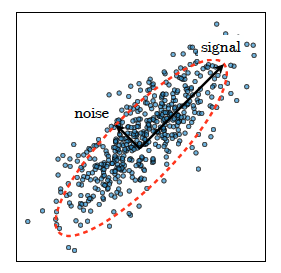
\includegraphics[scale =0.7]{images/PCA_var.png}	
	\caption{PCA seeks to find orthogonal directions with largest variance. Here, in 2D, the major axis of the ellipse corresponds to the first principal component, i.e. the direction with the highest variance, which is assumed to correspond to the true signal. The remaining direction is chosen to be perpendicular to the first, and it is assumed to corresponds to noise.}
\end{figure}





\section{Autoencoders}

Autoencoders are a type of neural network architecture that are primarily used for unsupervised learning and dimensionality reduction. They are designed to learn efficient representations of input data by compressing the input into a lower-dimensional latent space and then reconstructing the original input from this compressed representation.

\begin{figure}
	\centering
	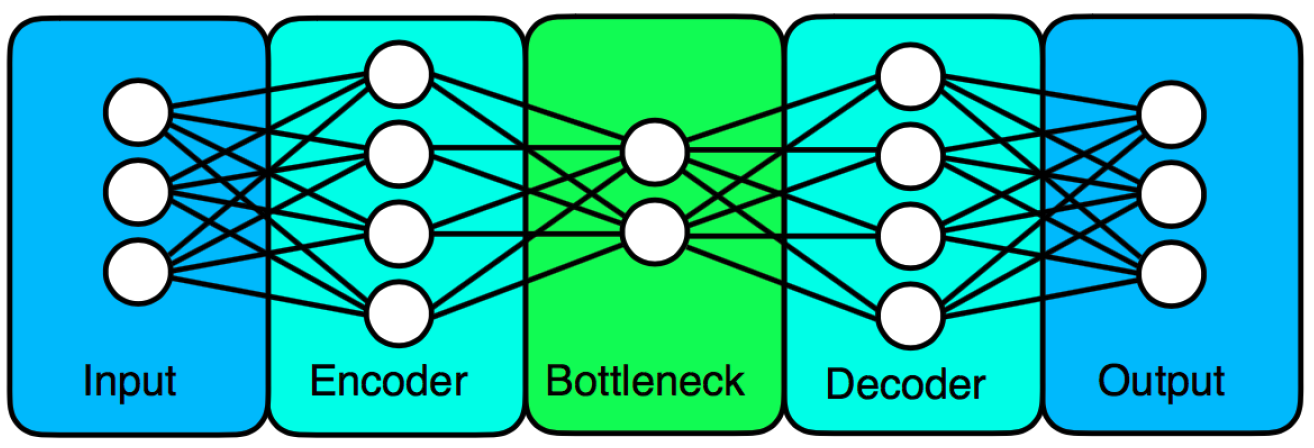
\includegraphics[scale = 0.5]{images/autoencoder.png}
	\caption{Architecture of a neural-network based autoencoder. The autoencoder finds a low-dimensional representation of the input, from which the decoder reconstructs an approximation of the input as output.}	
\end{figure}


In this work, the training data are the vectors $\bm{Q}(i)$ evaluated from snapshots of colloidal systems obtained via computer simulations, and the autoencoder is trained to find a low-dimensional projections of such vectors by eliminating irrelevant and redundant information. 

In the present context, we employ feedforward and fully connected autoencoders like in the figure. The number of input and output nodes, $d$ is specified by the dimensionality of the input vector $\bm{Q}(i)\in\mathbb{R}^d$, which are approximately reconstructed by the network in the output layer $\hat{\bm{Q}}(i)\in\mathbb{R}^d$. The bottleneck layer contains the low-dimensional projection to be learned by the encoder, $\bm{Y}(i)\in\mathbb{R}^c$, whose dimensionality is controlled by the number of bottleneck nodes, $c<d$. Nonlinearity is achieved by providing both the encoder and the decoder with a fully-connected hidden layer with a nonlinear activation function. Here, we set the number of nodes in the hidden layer to $10d$ and use a hyperbolic tangent as the activation function. For the bottleneck and output layers, instead, a linear activation function is used.


\subsection{Contribution Analysis}

ANNs have the capacity to predict output variable but the mechanisms that occur within the network are often ignored. ANNs are often considered as black boxes. Various authors have explored this problem and proposed algorithms to illustrate the role of variables in ANN models. Most works, however, study pruning methods, that is, methods that eliminate irrelevant input and reduce the size of the network. 

Even though good prediction and eliminating redundancy is desirable, knowing what contribution each variable makes is of prime importance as well. Contribution analysis uses methods to determine the influence of each input variable and its contribution to the output. They are not, therefore, pruning methods but procedures to estimate the relative contribution of each input variable. The methods that will interest us are the "input perturbation" and the "improved stepwise" methods. As we will see, both techniques require a single trained model, avoid having to repeat the training multiple times.

\subsubsection{Input Perturbation Method}

This method aims to assess the effect of small perturbations in each input of the neural network output. The algorithm adjusts the input values of one variable, by adding a perturbation, $x_i\rightarrow x_i + \delta$ with $\delta/x_i\in[0,0.5]$, while keeping the rest untouched. The aim is to assess the effect of small changes in each input on the neural network output, reflected in the cost function, say mean square error (MSE). In fact, the MSE of the neural network output is expected to increase as a larger amount of noise is added to the selected input variable. Wen can thus obtain a classification of the input variables by order of importance.

\subsubsection{Improved Stepwise Method}

Stepwise selection is an iterative process that starts with an empty model and incrementally adds or removes features based on certain criteria. The two main variations of stepwise selection are forward selection and backward elimination.

Forward selection: In this approach, the algorithm starts with an empty model and iteratively adds one feature at a time. At each step, the algorithm evaluates the performance of the model with the additional feature and selects the one that improves the model the most based on a predefined criterion (e.g., decrease in MSE). The process continues until no additional features improve the model.

Backward elimination: In this approach, the algorithm starts with a model containing all the features and removes one feature at a time. At each step, the algorithm evaluates the performance of the model after removing a feature and selects the one whose removal has the least impact on the model's performance based on the predefined criterion. The process continues until removing any additional feature significantly degrades the model's performance.

The stepwise method aims to strike a balance between model complexity and performance by selecting a subset of features that provides the best trade-off. This is essentially the classical stepwise method. Its major drawback is that after adding or removing an input, the network has to be trained again, being very inefficient. An improvement of this method consisted of building two others called improved stepwise method a and b, where only one model is used.






\chapter{Clustering}

\section{Gaussian Mixtures}

Gaussian Mixture Models (MDD) is a generative model used for modelling complex data distributions, and they are particularly useful for data clustering. 

MDD, being a generative model, aims to learn the underlying probability distribution of the input data. The basic assumption is that the data points within each cluster are generated from a multivariate Gaussian distribution. A multivariate gaussian distribution is characterised by its mean vector and covariance matrix, which capture the location and shape of the distribution, respectively.

GMMs combine multiple Gaussian distributions to form a mixture model. Each gaussian distribution represents a component or cluster within the data. The mixture model specifies the proportions or weights of each component, indicating the contribution of each component to the overall distribution.

The goal of GMM training is to estimate the model parameters (means, covariance matrices and weights) that best fit the observed data. One such algorithm is the Expectation Maximisation (EM) algorithm. The EM algorithm is commonly used to iteratively estimate the parameters of a GMM. It consists of two main steps: the expectation step (E-step) and the Maximisation step (M-step). In the E-step, the algorithm computes the posterior probabilities of each data point belonging to each component. In the M-step, the algorithm updates the parameters of each Gaussian component based on the computed posteriors.

Once the GMM is trained and the parameters are estimated, it can be used for various tasks. For clustering, each data point is assigned to the component with the highest responsibility, indicating the cluster it belongs to. 

\subsection{EM Algorithm}

The EM algorithm is an iterative procedure designed to estimate the parameters in models with missing or incomplete data. It is particularly useful when the missing data introduces uncertainty or when dealing with latent variables.

The EM algorithm is a powerful technique for likelihood maximization in the presence of missing data. It effectively handles situations where direct maximization of the likelihood is not possible. By iteratively estimating the missing values and updating the parameters, the EM algorithm converges to a local maximum of the expected log-likelihood function. However, it does not guarantee convergence to the global maximum, and the algorithm may get stuck in suboptimal solutions.

Latent variables:
In some models, there are unobserved or latent variables that influence the observed data. These latent variables are not directly observed, but they play a crucial role in the underlying model. 

\subsection{Finding the number of clusters}

The simplest form of clustering that can be applied with GMMs consists in considering each mixture component as generating a separate cluster and assigning each observation to the component with the highest posterior probability. However, while this procedure works perfectly for clusters that are really generated from a mixture of separate multivariate normal distributions, the clusters that underline our data are very often far from being Gaussian-distributed in space. As a consequence a single cluster in the data may be detected as two or more mixture components (if its distribution is indeed better approximated by a mixture of Gaussians than by a single Gaussian function), meaning that the number of clusters in the data may in general be different from the number of components by minimising the BIC.

[Reference] argues that the goal of selecting the number of mixture components for estimating the underlying probability density is well met by BIC, but that the goal of selecting the number of clusters may not be. Even when a multivariate Gaussian mixture model is used for clustering the number of mixture components is not necessarily the same as the number of clusters. This is because a cluster may be better represented by a mixture of normals than by a single normal distribution.

BIC is used to select the number of components in the mixture model. They then propose a sequence of possible solution by a hierarchical combination of the components identified by BIC. 
The dicision about which components to combine is based on minimising the entropy of the resulting clustering define as
\begin{align}
	S_K=-\sum_{i=0}^N\sum_{j=1}^K p_{ij}\ln(p_{ij})
\end{align}
where $N$ is the number of observations and $K$ is the number of clusters. Practically, the optimal number of 


\chapter{Simulations}

\section{Square-shoulder particles in 2D}


The square shoulder potential is given by
\begin{align}
	U(r_{ij})=\left\{
	\begin{aligned}
		&\infty \qquad\qquad && r_{ij}\leq L\\
		&\sigma &&L<r_{ij}\leq\lambda L\\
		&0 && r_{ij}>\lambda L
	\end{aligned}
	\right.
\end{align}

\end{document}